\documentclass[a4paper,11pt]{article}
\usepackage[utf8]{inputenc}
\usepackage[spanish, es-tabla]{babel}
\usepackage{amsmath}
\usepackage{amsfonts}
\usepackage[pdftex]{graphicx}
\usepackage[table]{xcolor}
\usepackage{subfigure}
\numberwithin{equation}{section}
\setcounter{secnumdepth}{5}
\usepackage{cancel}
\usepackage[margin=2cm,font=footnotesize,labelfont=bf]{caption} 
\usepackage{booktabs}
\usepackage{titlesec}
\usepackage{cite}
\usepackage[numbered,framed]{mcode}
\usepackage{float}
\usepackage[nottoc]{tocbibind} %Para poner bibliografia en el Indice





\begin{document}
	\titleformat*{\section}{\LARGE\bfseries}
	\titleformat*{\subsection}{\Large\bfseries}
	\titleformat*{\subsubsection}{\large\bfseries}
	\titleformat*{\paragraph}{\large\bfseries}
	\titleformat*{\subparagraph}{\large\bfseries}
	\renewcommand{\(}{\left(}
	\renewcommand{\)}{\right)}
	\newcommand{\espacio}{\hspace{0.5cm} \Rightarrow \hspace{0.5cm}}
\begin{titlepage}
	\begin{figure}[ht]
		\flushright
		\vspace{-2.3cm}
		
\includegraphics[width=3cm]{logo}
	\end{figure}
	\vspace{0.5cm}
	\begin{center}
		\large{Universidad de Córdoba\\	
			Facultad de Ciencias - Grado de Física} 
		
		\vspace{2cm}
		\textbf{\Large 14. PROPAGACIÓN DE UNA ENFERMEDAD INFECCIOSA}
		\vspace{5cm}
		\vspace{1cm}\\
		{\Large Métodos Numéricos y Simulación\\	\vspace{10pt}
			2º Curso \\
			2014-2015}
		
		\vspace{2cm} 
		\begin{center}
			\textbf{Realizado por:}\\	
			Eros Camacho Ruiz\\
		\end{center}
		\vspace{4cm}
	\end{center}
\end{titlepage}
\newpage
\tableofcontents
\newpage
\section{Introducción}

\indent Desde que el ser humano se encuentra en la Tierra uno de los grandes problemas que siempre ha surgido son las enfermedades, en concreto las enfermedades infecciosas. Existen factores en la propagación de una enfermedad infecciosa que muchas veces no tenemos en cuenta, como por ejemplo, la higiene de los individuos o incluso eventos ocasionales como terremotos o inundaciones que dificultan aún más la labor de los sanitarios a la hora de controlar esa enfermedad. Enfermedades como la peste negra durante el siglo XIV se cobraron la vida de más de 34 millones de personas{\tiny \bf \textsuperscript{\cite{wikiuno}}}. Hecho que se podría haber evitado si se hubieran contado con los medios adecuados. 
\\

\indent Es por ello, que el uso de métodos matemáticos, en concreto de métodos numéricos para estudiar la dinámica de transmisión de una enfermedad infecciosa ha cobrado vital importancia. Un modelo matemático que te describa previamente de qué manera va a comportarse dicha enfermedad permite no sólo ganar tiempo para combatirla, sino que también permite salvar vidas.  \\

\indent En este trabajo se exponen varios modelos numéricos que predicen de un manera muy aproximada el comportamiento de dicha enfermedad en una población determinada, obteniendo un número de población infectada infectada en un tiempo determinado{\tiny \bf \textsuperscript{\cite{blog}}}. Se puede comprobar que siguen comportamientos de casos reales, que también comentaremos.

\newpage
\section{Análisis del problema}
\indent Como hemos mencionado la idea principal es la de obtener el número de infectados que aparecen en una población cuando aparece una enfermedad infecciosa. En la teoría de propagación de una enfermedad infecciosa surge la idea de utilizar una ecuación diferencial{\tiny \bf \textsuperscript{\cite{hoja}}} que satisfaga unos resultados esperados, haciendo ciertas consideraciones anteriores a abordar el problema que se nos plantea. 

\subsection{Enfermedad sin eliminación de la población}
\indent En este primer caso vamos a suponer que los individuos en una población fija tienen las mismas probabilidades de contagio, y que los ya contagiados permanecerán en ese estado. Denotaremos $ x(t) $ al número de individuos que aún no han sido contagiados e $ y(t) $ a los que han contraído la enfermedad. Como puede observarse dependen de un tiempo $ t $ cuyas unidades para la elaboración de nuestro problema van a ser días. Como $ x(t) $ representa los que están sanos e $ y(t) $ los que no podemos determinar la población total $ m $ del siguiente modo{\tiny \bf \textsuperscript{\cite{hoja}}}:
\begin{equation}
x(t)+y(t)=m
\label{eq:pob1}
\end{equation}

\indent Es razonable suponer que la tasa con la que varía la población infectada con respecto del tiempo debe ser proporcional al número de $ x(t) $ e $ y(t) $ ya que esta tasa depende tanto del número de contagiados como del número de los que aún están sanos. Si se supone una población demasiado grande como para que $ x $ e $ y $ sean variables continuas, el problema puede expresarse del siguiente modo{\tiny \bf \textsuperscript{\cite{hoja}}}: 
\begin{equation}
\frac{dy}{dt}=kyx
\label{eq:dif1}
\end{equation}

\indent Donde $ k $ es una constante{\tiny \bf \textsuperscript{\cite{hoja}}} que puede relacionarse con una tasa de infección que en nuestro caso es un valor dado, pero que en otro caso puede ser calculada mediante un ajuste lineal de datos. Si tomamos ahora la Ecuación \ref{eq:pob1} y despejamos $ x(t) $ tenemos que:
\begin{equation}
x(t)=m-y(t)
\label{eq:pob2}
\end{equation}

\indent Si ahora sustituimos la Ecuación \ref{eq:pob2} en la Ecuación \ref{eq:dif1} tenemos que:
\begin{equation}
\boldsymbol{\frac{dy}{dt}=ky(m-y)}
\label{eq:dif2}
\end{equation}

\indent Así obtenemos una Ecuación en términos de $ y(t) $ que una vez resuelta nos dará el numero de infectados por unidad de tiempo{\tiny \bf \textsuperscript{\cite{hoja}}}. \\

\indent Como vemos es una ecuación de tipo logística cuya forma general tiene la siguiente expresión{\tiny \bf \textsuperscript{\cite{wikidos}}}:

\begin{equation}
P(t)=\frac{1}{1+e^{-t}}
\label{eq:logis}
\end{equation}

\indent Este tipo de ecuaciones se utiliza en el modelado y crecimiento de poblaciones, rumores, impactos tecnológicos, crecimiento de células e incluso enfermedades. Es por ello que este problema que nos planteamos se resuelva con ecuaciones de este tipo. \\
 
\indent El método de resolución de nuestro problema en este caso va a ser la utilización de métodos numéricos, sin embargo también puede ser calculada utilizando métodos analíticos, recordando que la Ecuación \ref{eq:dif2} se trata de una \textit{ecuación de Bernouilli}. Para ello hacemos el siguiente cambio:
\begin{equation}
u=y^{-1}
\label{eq:resolver1}
\end{equation}

\indent De donde podemos hacer las siguientes operaciones:
\begin{equation}
y=u^{-1} \espacio \frac{dy}{dt}=-u^{-2}\frac{du}{dt}
\label{eq:resolver2}
\end{equation}

\indent Utilizando lo obtenido en la Ecuación \ref{eq:resolver2} en la Ecuación \ref{eq:dif2} tenemos que:
\begin{equation}
y'=kmy-ky^2 \espacio -u^{-2}u'=kmu^{-1}-ku^{-2}
\label{eq:resolver3}
\end{equation}

\indent Continuando con las operaciones tenemos que:
\begin{equation}
u'=k-kmu=k(1-mu)
\label{eq:resolver4} 
\end{equation}

\indent Obteniendo una Ecuación Diferencial Ordinaria:
\begin{equation}
\frac{du}{1-mu}=kdt
\label{eq:resolver5}
\end{equation}

\indent De ese modo procedemos a integrar la Ecuación \ref{eq:resolver5} obteniendo:
\begin{equation}
 \frac{-1}{m}\ln(1-mu)=kt+C
 \label{eq:resolver6}
\end{equation}

\indent De donde después de hacer operaciones y deshacer el cambio de $ u $ obtenemos:
\begin{equation}
\boldsymbol{y=\frac{m}{1+Ce^{-mkt}}}
\label{eq:resolver7}
\end{equation}

\indent Como vemos se trata de una ecuación de tipo exponencial. Para ver si el resultado que hemos obtenido coincide con la realidad, recordemos que en un tiempo infinito la enfermedad teóricamente se habrá propagado a toda la población, pues no hemos considerado que exista cura ni que se produzcan muertes u otros efectos. Por lo que si estudiamos el límite de la Ecuación \ref{eq:resolver7}, obtenemos que:

\begin{equation}
\lim\limits_{t\rightarrow\infty} \frac{m}{1+Ce^{-mkt}} = \frac{m}{1+0}=m
\label{eq:limite}
\end{equation}

\indent Atendiendo a lo obtenido en la Ecuación \ref{eq:limite}, como observamos, los resultados teóricos coinciden con la realidad. Cuando consideramos un tiempo infinito toda la población ha sido contagiada por la enfermedad.

\subsection{Enfermedad con eliminación de la población}

\indent Mientras que en el caso anterior, todos los individuos contagiados permanecían en la población y esparcían así la enfermedad. En este caso vamos a considerar que existen individuos que se eliminan de la población ya sea por aislamiento, recuperación, inmunidad o muerte. Así introducimos una nueva variable,  $ z(t) $, que representa el número de individuos que se eliminan de la población en un tiempo $ t $ determinado. Al igual que el caso anterior $ x(t) $ representa los individuos sanos e $ y(t) $ los individuos que han contraído la enfermedad en una población $ m $ que este vez se define como:
\begin{equation}
x(t)+y(t)+z(t)=m 
\label{eq:pob3}
\end{equation} 

\indent El tasa de eliminación de individuos por unidad de tiempo debe ser proporcional a una constante $ k_2 $ denominada \textit{constante de eliminación de individuos} y al número de infectados, por lo que podemos plantear la siguiente ecuación diferencial:
\begin{equation}
\frac{dz}{dt}=k_2y;
\label{eq:edo1}
\end{equation}

\indent De la Ecuación \ref{eq:pob3} podemos despejar $ y(t) $ obteniendo:
\begin{equation}
y(t)=m-x(t)-z(t)
\label{eq:pob4}
\end{equation}

\indent Así podemos sustituir $ y(t) $ en la Ecuación \ref{eq:edo1}, obteniendo:
\begin{equation}
\frac{dz}{dt}=k_2(m-x-z)
\label{eq:edo2}
\end{equation}

\indent Por otro lado, se demuestra que $ x(t) $ tiene la siguiente expresión, donde $ k_1 $ representa la \textit{tasa de infección}:
\begin{equation}
x(t)=x(0)e^{-(k_1/k_2)z(t)}
\label{eq:x1}
\end{equation}

\indent Sustituyendo la Ecuación anterior en la Ecuación \ref{eq:edo2} obtenemos que:
\begin{equation}
\frac{dz}{dt}=k_2(m-z-x(0)e^{-(k_1/k_2)z})
\end{equation}

\indent Esta ecuación no tiene un método de resolución analítico, por lo que nuestra única opción es la de obtener una solución aproximada utilizando métodos numéricos.
 
\section{Metodología de resolución}
\indent En este caso se nos plantea la resolución de una \textit{Ecuación Diferencial}, cuya solución analítica es fácil de obtener (Ecuación \ref{eq:resolver7}). Pero nuestro problema se nos plantea en el ámbito del cálculo numérico, por lo que tendremos que utilizar algún método numérico destinado a su resolución. En concreto este problema es un problema denominado \textit{problema de valores iniciales} o simplemente \textit{PVI}, puesto que se nos imponen condiciones de partida. Su finalidad es la de determinar la constante de integración que aparece en nuestro problema. Se plantean del siguiente modo:
\begin{equation}
t_0=0 \espacio y(t_0)=y_0
\label{eq:met1}
\end{equation}

\indent Para el caso de \textit{Enfermedad sin eliminación de la población} vamos a utilizar un método numérico denominado \textit{Método de Runge-Kutta de orden 4}. Es un método que no sólo tiene un error del orden de $ h^4 $ sino que cuenta con una rápida convergencia sin tener que tomar $ h $ demasiado pequeño.{\tiny \bf \textsuperscript{\cite{hoja2}}}\\

\indent Para este caso vamos a utilizar las siguientes variables:
\begin{itemize}
	\item $ \boldsymbol{k} $ : Tasa de contagio
	\begin{equation}
	k=2\cdot 10^{-6}
	\end{equation}
	\item $ \boldsymbol{m} $ : Población
	\begin{equation}
	m=100000
	\end{equation}
	\item $ \boldsymbol{y_0} $ : Número de contagiados inicialmente
	\begin{equation}
	y_0=1000
	\end{equation}
\end{itemize}

\indent Para el caso de \textit{Enfermedad con eliminación de la población} vamos a utilizar un método numérico denominado \textit{Método de Heun} o \textit{Método de Euler mejorado}. Este método es una versión del \textit{Método de Euler} que mejora en el cálculo de la integral, utilizando el denominado método del trapecio. Pierde precisión con respecto al \textit{Método de Runge-Kutta de orden 4} pero cuenta con una rápida convergencia que nos permite obtener valores rápidamente que podemos comparar con los resultados numéricos obtenidos en el cálculo de la \textit{Enfermedad sin eliminación de la población}.{\tiny \bf \textsuperscript{\cite{hoja2}}} \\

\indent Para este caso vamos a utilizar las siguientes variables:
\begin{itemize}
	\item $ \boldsymbol{k_1} $ : Tasa de contagio
	\begin{equation}
	k_1=2\cdot 10^{-6}
	\end{equation}
	\item $ \boldsymbol{k_2} $ : Constante de eliminación de individuos
	\begin{equation}
	k_2=1\cdot 10^{-4}
	\end{equation}
	\item $ \boldsymbol{m} $ : Población
	\begin{equation}
	m=100000
	\end{equation}
	\item $ \boldsymbol{y_0} $ : Número de contagiados inicialmente
	\begin{equation}
	y_0=1000
	\end{equation}
	\item $ \boldsymbol{z_0} $ : Número de población eliminada inicialmente
	\begin{equation}
	z_0=0
	\end{equation}
\end{itemize}

\section{Códigos}
\indent A continuación expongo los códigos empleados en la realización de este trabajo.

\subsection{Enfermedad sin eliminación de la población}
\indent Código correspondiente al archivo \texttt{trabajo\_optativo1.m}
\lstinputlisting{trabajo_optativo1.m}

\newpage
\subsection{Método Runge-Kutta de orden 4 modificado}
\indent Código correspondiente al archivo \texttt{RK4\_to.m}
\lstinputlisting{RK4_to.m}

\subsection{Enfermedad con eliminación de la población}
\indent Código correspondiente al archivo \texttt{trabajo\_optativo2.m}
\lstinputlisting{trabajo_optativo2.m}

\subsection{Método de Heun modificado}
\indent Código correspondiente al archivo \texttt{heunsis\_to.m}
\lstinputlisting{heunsis_to.m}

\subsection{Comparación entre los dos problemas}
\indent Código correspondiente al archivo \texttt{trabajo\_optativo3.m}
\lstinputlisting{trabajo_optativo3.m}

\subsection{Comentarios acerca de los programas}
\indent En esta sección quiero dejar claro algunos problemas que surgieron a la hora de llevar a cabo la programación de los problemas planteados.
\begin{itemize}
	\item Con respecto a la programación de los problemas y la implementación de los métodos estudiados ha sido muy sencilla en parte. El único problema que se ha encontrado ha sido en la llamada de las variables y en la modificación de los métodos numéricos escritos para su correcto funcionamiento en nuestro problema. Una vez que estos problemas fueron solventados no se encontró ningún problema añadido.
	\item Con respecto al primer problema que se nos plantea y al de un caso práctico que estudiaremos más adelante, se encontraron ciertos problemas de estabilidad al variar alguno de los parámetros de entrada (tasa de infección o población). Al modificarlos se generaban valores muy divergentes, por lo que siendo un buen método para resolver este tipo de problemas sólo presenta convergencia para ciertos valores que están estrechamente relacionados. 
	\item La determinación del número de iteraciones ($ n $) para el primer problema fue determinada mediante una prueba de ensayo y error comparando los resultados obtenidos con el resultado real. Un número de 20 iteraciones consideramos que hubiera sido válido, pero puesto que no nos supone mucho tiempo de procesamiento, se optó por tomar 30 iteraciones aumentando la precisión de los resultados obtenidos. Para el segundo caso, puesto que no conocemos el valor de la solución real consideramos que con 50 iteraciones se conseguía suficiente precisión como para poder realizar cálculos y estimaciones.
\end{itemize}

\newpage
\section{Resultados numéricos}
\indent A continuación expongo los resultados numéricos que se obtuvieron a la hora de resolver los problemas que se nos plantean.
\subsection{Enfermedad sin eliminación de la población}
\indent Con respecto a esta parte, lo primero que se hizo fue representar los valores que se obtienen por un lado de la solución analítica y por otro los de la solución numérica, con el fin de compararlos más adelante y poder obtener conclusiones.
\begin{figure}[h!]
		\centering 		
		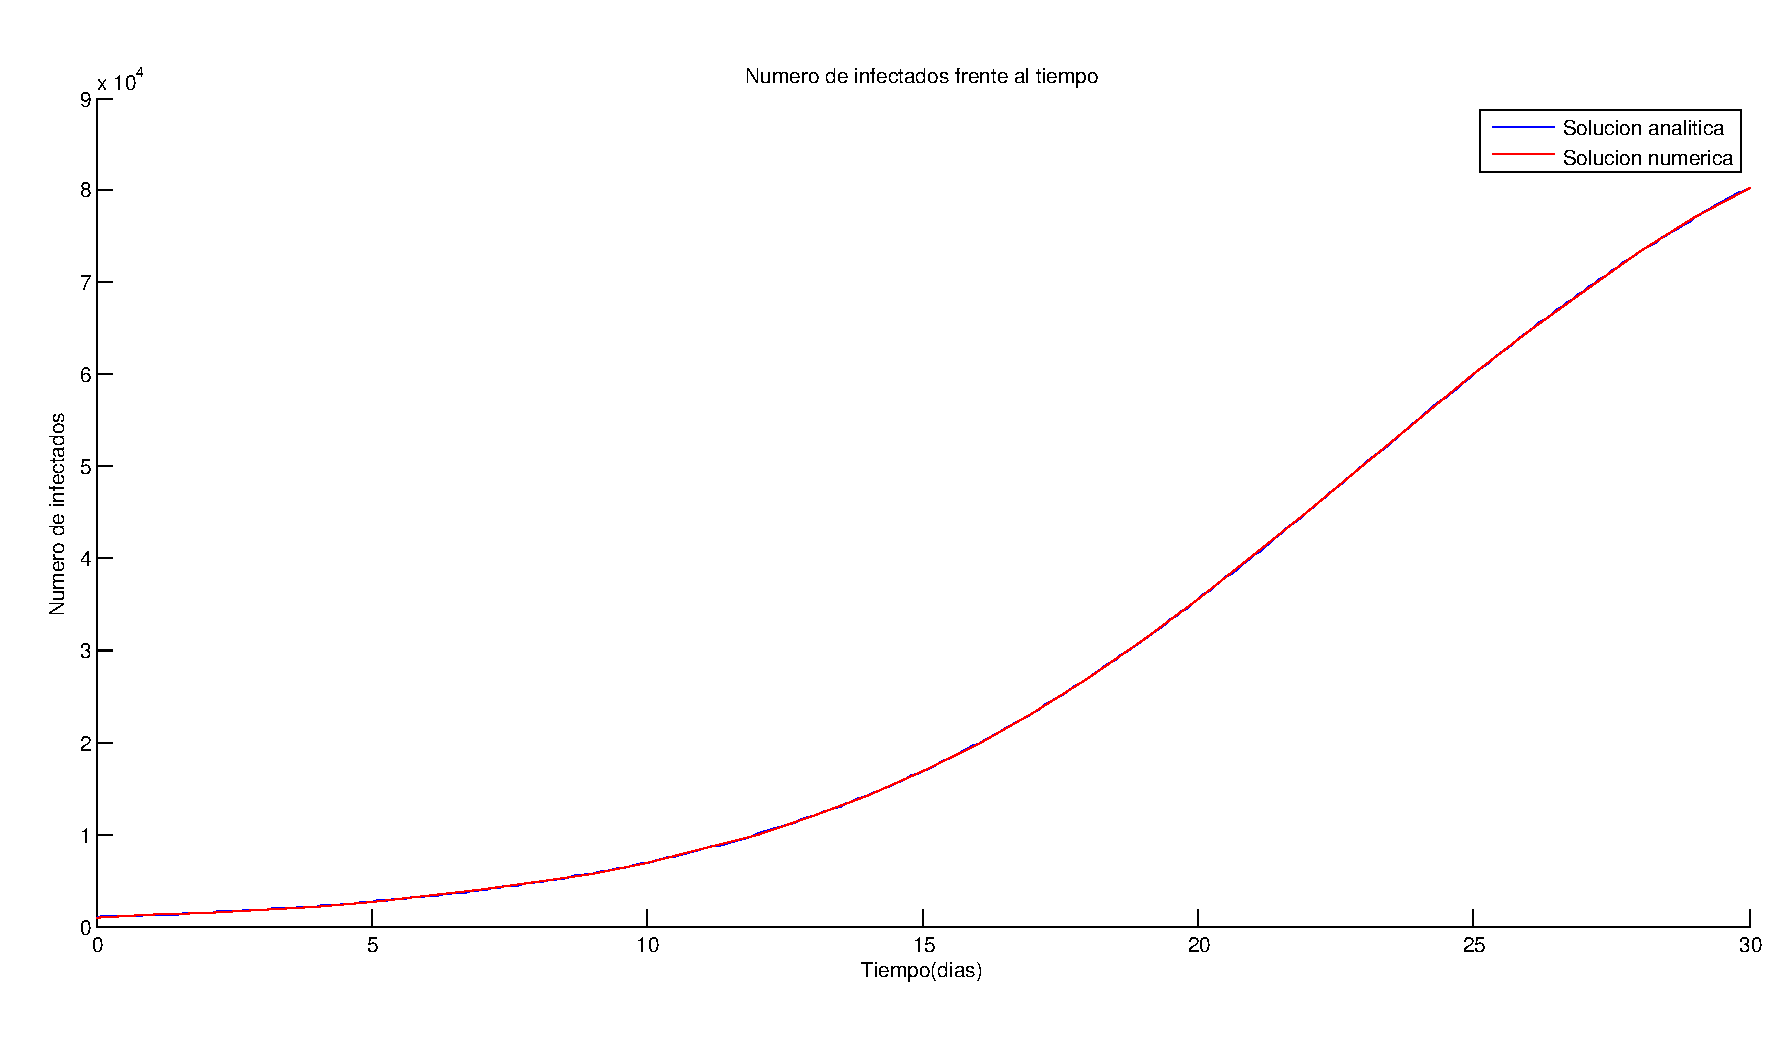
\includegraphics[width=1\textwidth]{grafica1.pdf}
		\caption{Número de infectados frente al tiempo}
		\label{Fig:1}
\end{figure}

\indent Obteniendo para el caso de la solución analítica $ 80296 $ personas infectadas en 30 días, mientras que para la solución numérica obtenemos $ 80295 $ personas. \\

\indent A continuación lo que se hizo fue representar la población total y ver en cada momento la cantidad de personas que se encuentran infectadas y las que aún se mantienen sanas. Como en la anterior gráfica los resultados que se obtienen son muy parecidos, consideré separar las gráficas para que se pudiera apreciar con mucho más detalle la tendencia que se sigue.

\begin{figure}[h!]
	\centering 		
	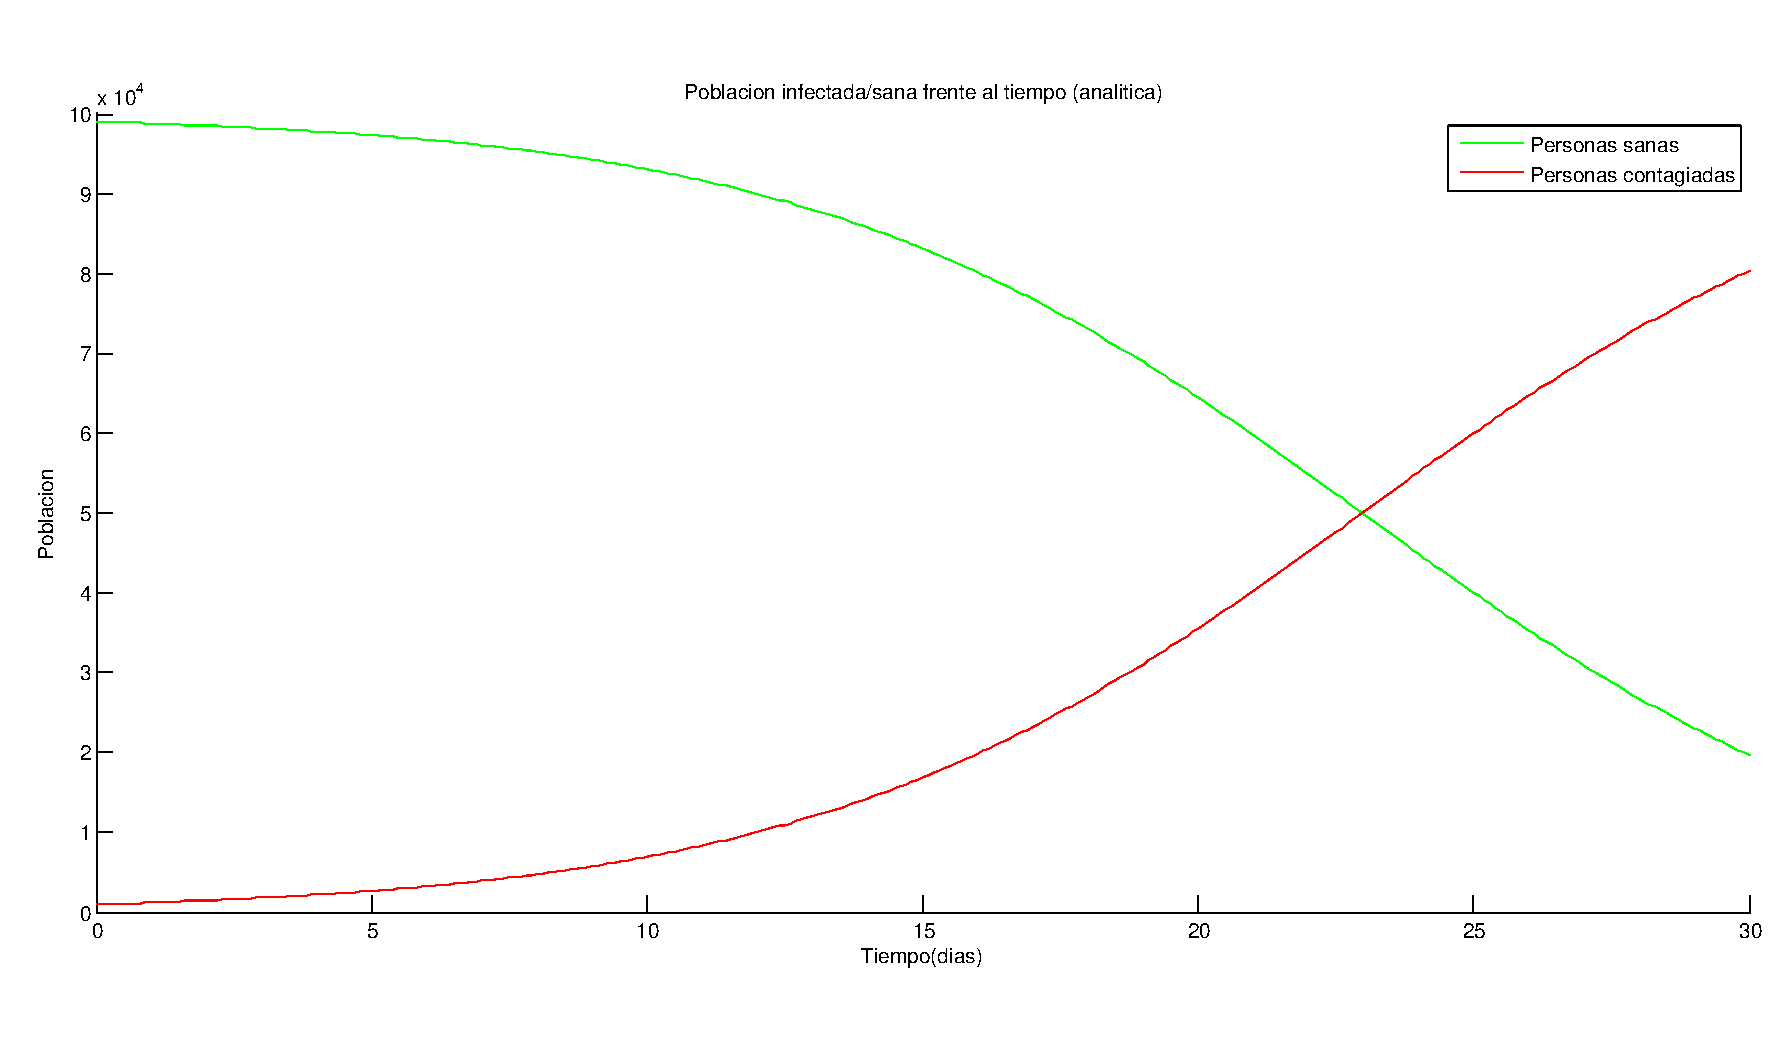
\includegraphics[width=1\textwidth]{grafica2.pdf}
	\caption{Población infectada/sana frente al tiempo (solución analítica)}
	\label{Fig:2}
\end{figure}

\indent Del mismo modo que antes se obtienen $ 80296 $ personas infectadas en 30 días, mientras que $ 19704 $ aún siguen sanas.

\begin{figure}[h!]
	\centering 		
	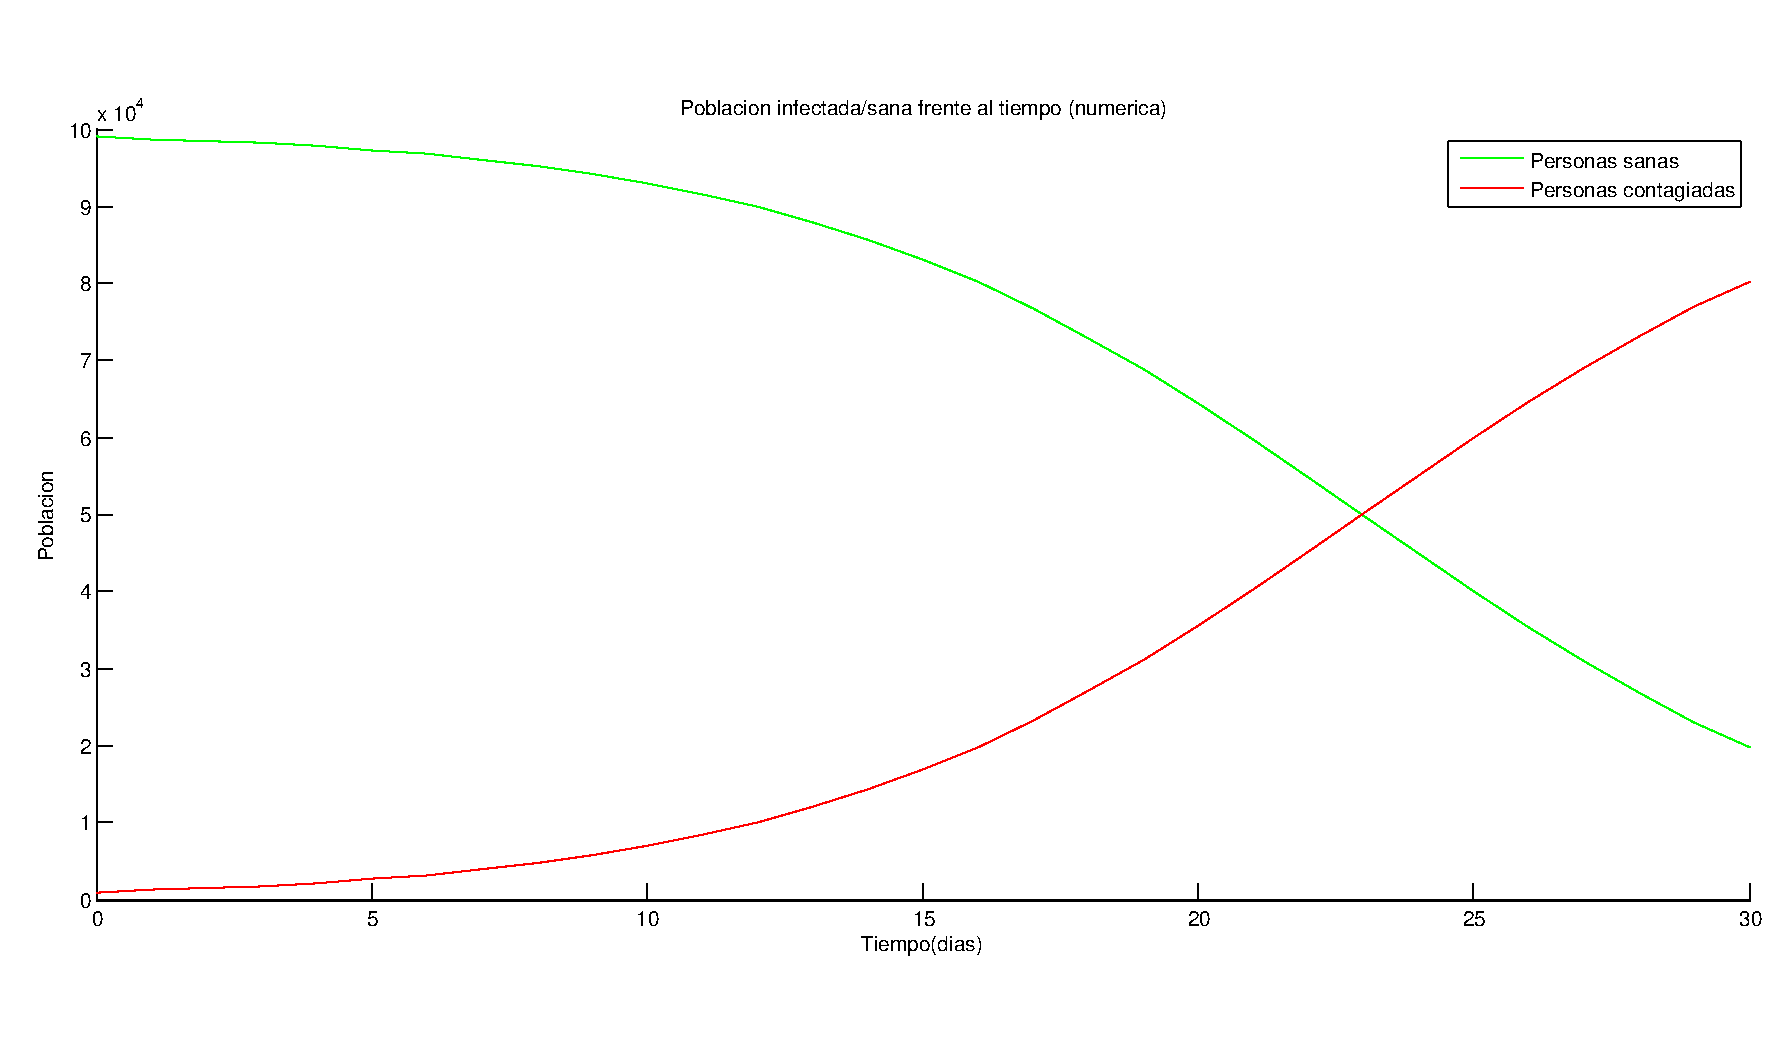
\includegraphics[width=1\textwidth]{grafica3.pdf}
	\caption{Población infectada/sana frente al tiempo (solución numérica)}
	\label{Fig:3}
\end{figure}

\newpage
\indent Del mismo modo que antes se obtienen $ 80295 $ personas infectadas en 30 días, mientras que $ 19705 $ aún siguen sanas.

\subsection{Enfermedad con eliminación de la población}
\indent Con respecto a esta parte, lo primero que se hizo fue representar la población que se eliminaba a causa de la enfermedad contagiosa frente al tiempo. \\
\begin{figure}[h!]
	\centering 		
	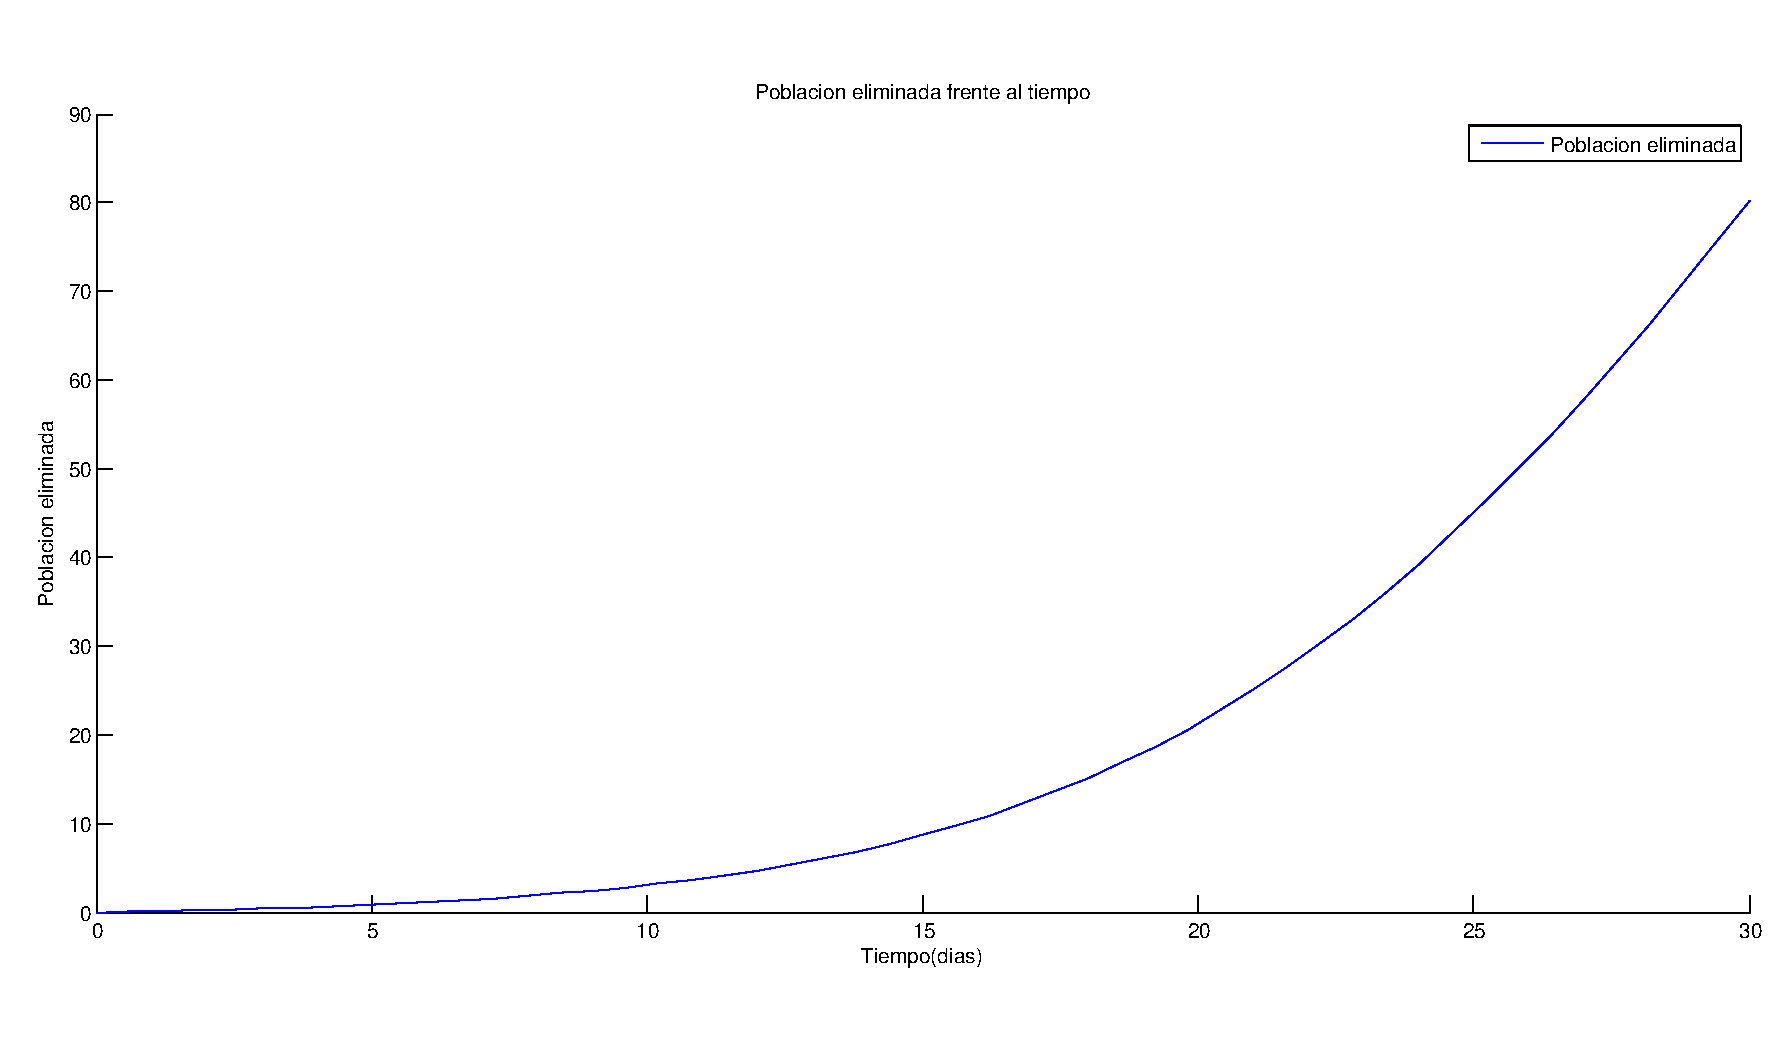
\includegraphics[width=1\textwidth]{grafica4.pdf}
	\caption{Población eliminada frente al tiempo}
	\label{Fig:4}
\end{figure}

\indent De ese modo se obtienen $ 80 $ personas de la población que se han curado, son inmunes o simplemente han fallecido en un total de 30 días. \\

\indent En la siguiente gráfica recojo los valores de personas sanas y personas que han contraído la enfermedad. Puesto que el valor de personas que se eliminan es sustancialmente más pequeño que los valores de población infectada y sana no aparece en esta gráfica. Los valores son tan pequeños que no se aprecia la diferencia de población. Notemos que en este caso la población que sobrevive es la suma de la población infectada y la población sana. La población eliminada se elimina del total inicial.\\
\begin{figure}[h!]
	\centering 		
	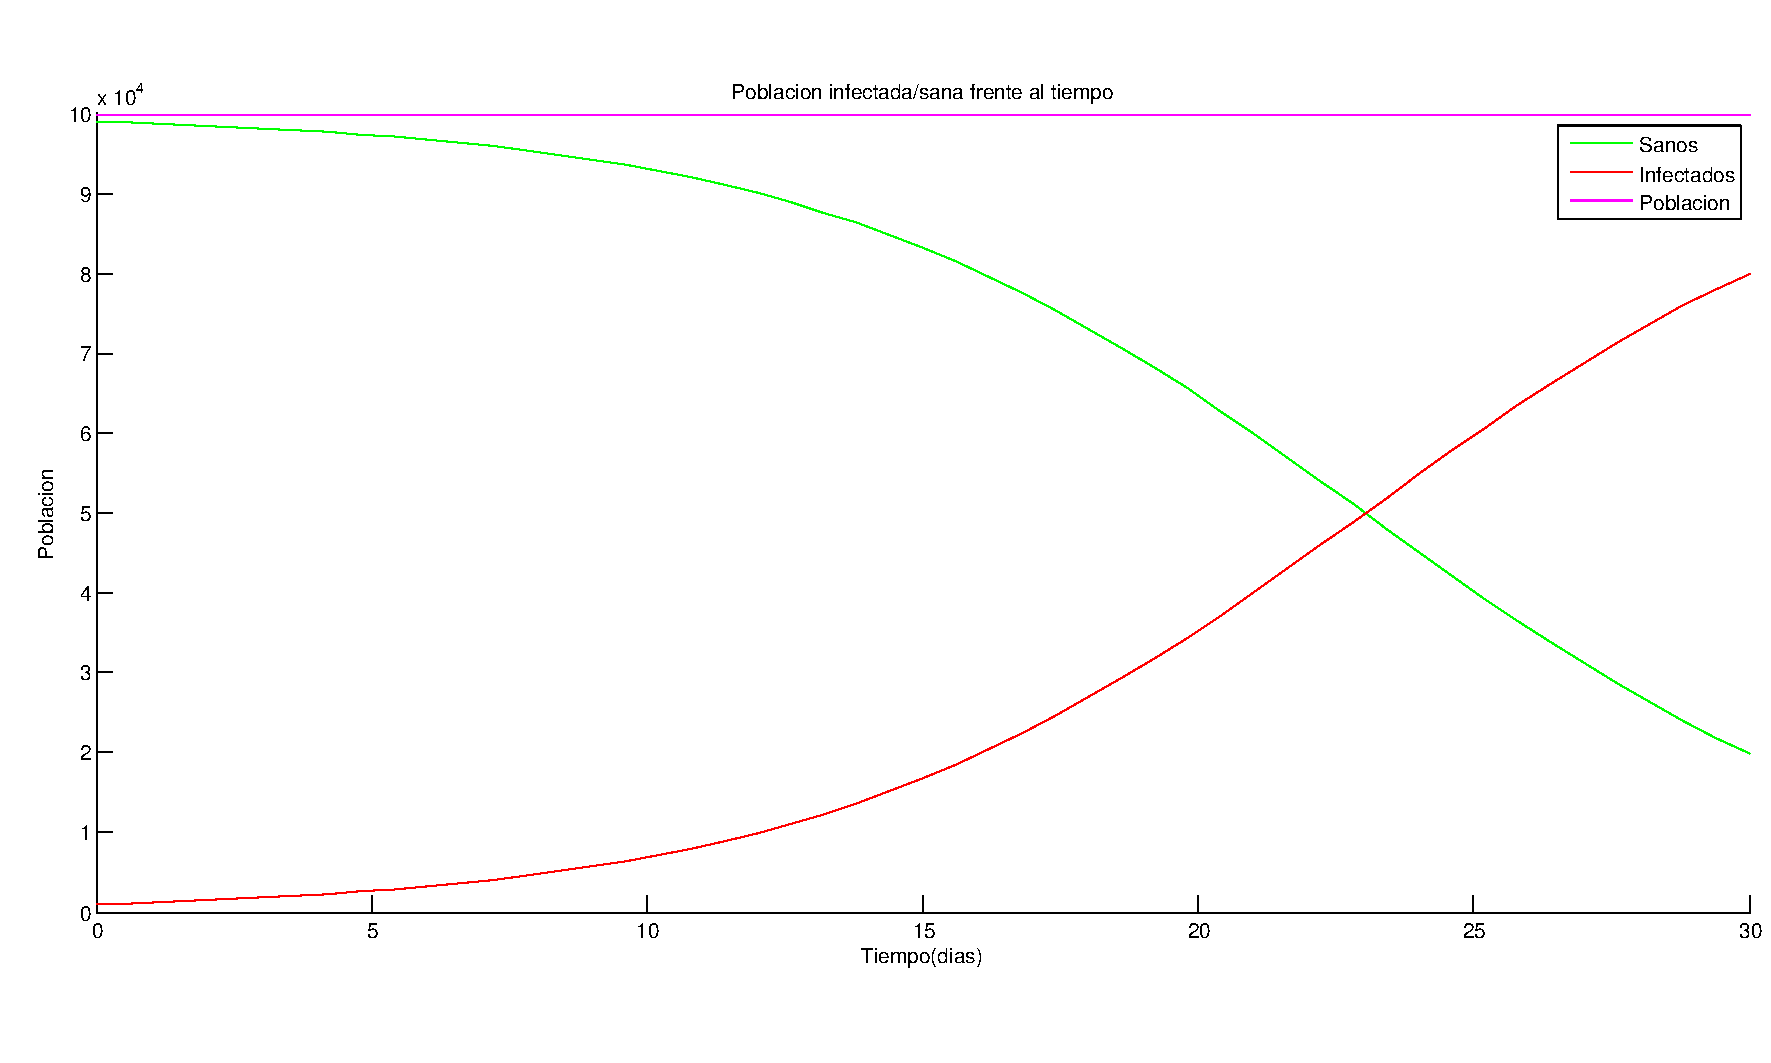
\includegraphics[width=1\textwidth]{grafica5.pdf}
	\caption{Población infectada/sana frente al tiempo}
	\label{Fig:5}
\end{figure}

\newpage
\indent Obteniendo en este caso $ 80025 $ personas infectadas en 30 días, mientras que $ 19895 $ aún siguen sanas. Como puede observarse la población a considerar a disminuido. Al cabo de 30 días se obtiene una población de $ 99920 $ personas, faltando las $ 80 $ personas que han sido predecidas por $ z(t) $.

\subsection{Comparación entre los dos problemas}
\indent Puesto que como hemos dicho en el anterior caso los valores de población eliminada son apenas imperceptibles la única solución que nos queda es la de representar los dos problemas en una misma gráfica y observar la diferencia de valores que se obtiene. \\
\begin{figure}[h!]
	\centering 		
	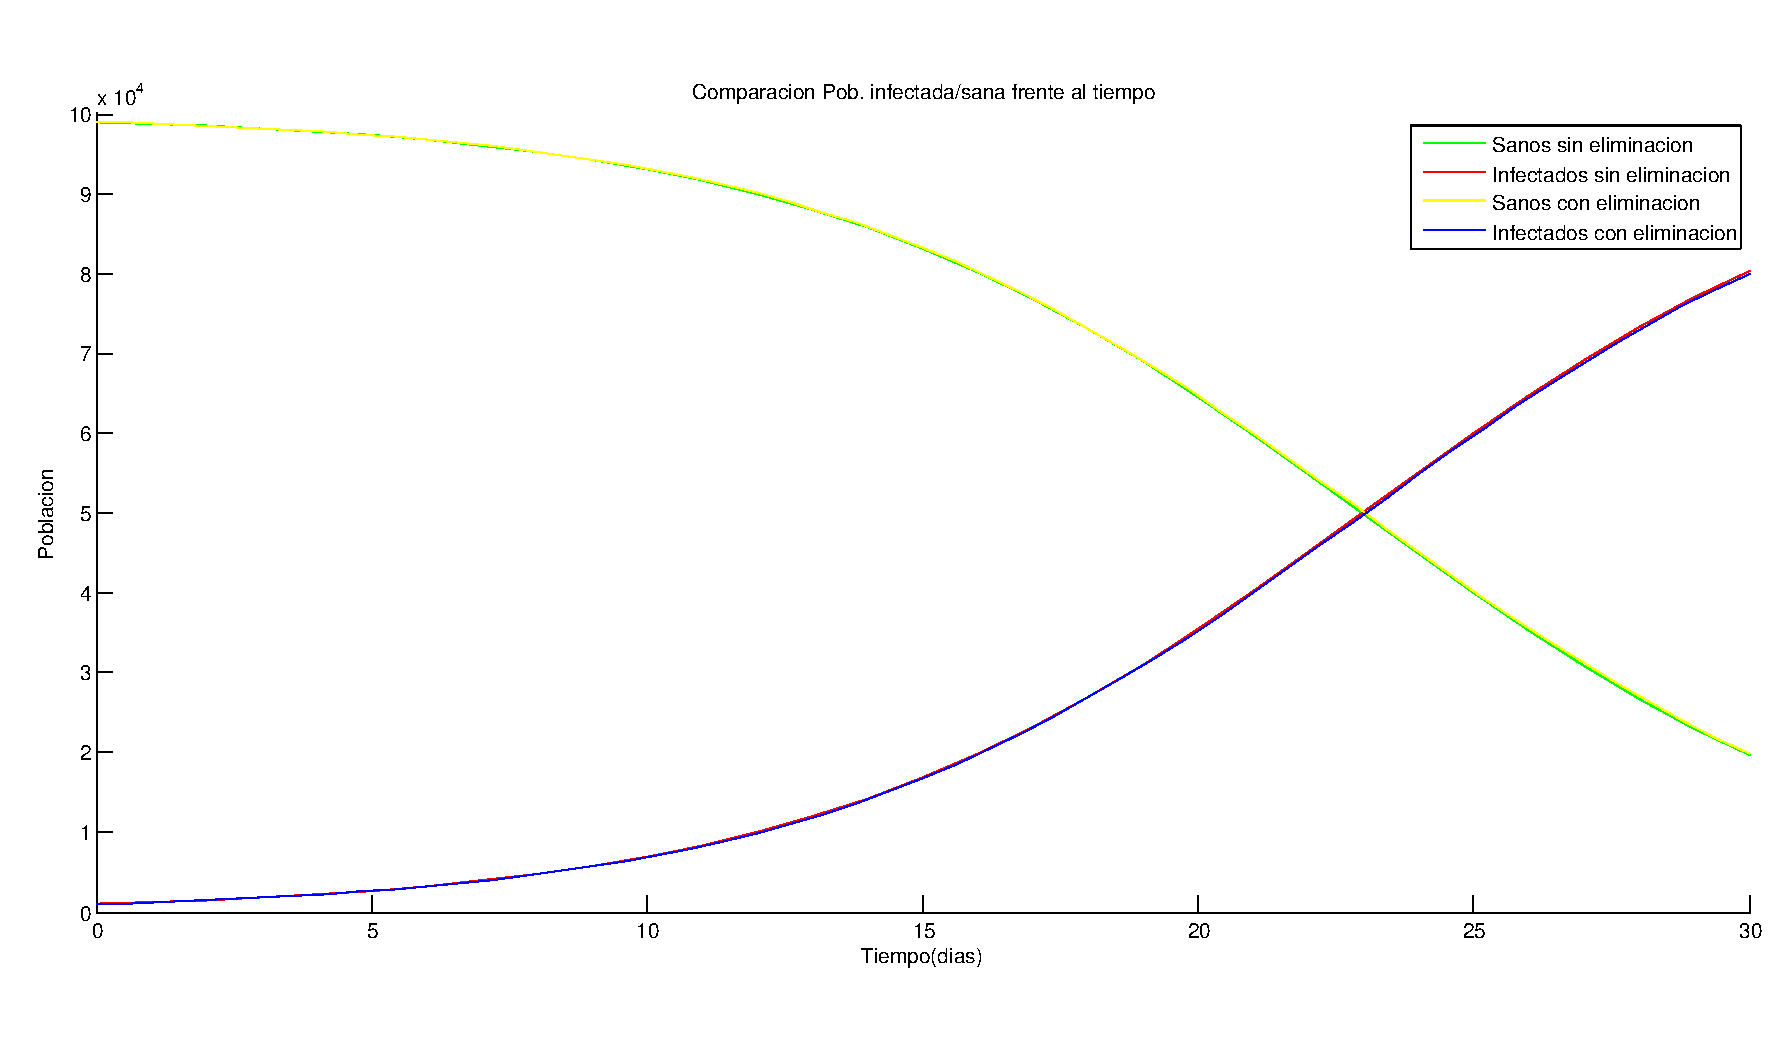
\includegraphics[width=1\textwidth]{grafica6.pdf}
	\caption{Comparación población infectada/sana frente al tiempo}
	\label{Fig:6}
\end{figure}

\newpage
\indent En este caso los valores que se obtienen a los 30 días son los mismos que se han obtenido en los anteriores cálculos. Así podemos determinar la diferencia de personas entre un caso y otro (solamente vamos a considerar el caso numérico). Para personas contagiadas existe una diferencia de $ 270 $ personas, mientras que para personas sanas existe una diferencia de $ 190 $ personas. 

\section{Análisis de resultados obtenidos}
\indent A continuación se detallan de forma pormenorizada un análisis de los resultados obtenidos.
\subsection{Enfermedad sin eliminación de la población}
\indent Como hemos mencionado anteriormente, lo primero que se hizo fue obtener una expresión de la solución analítica integrando la Ecuación \ref{eq:dif2}, obteniendo la Ecuación \ref{eq:resolver7}. Por otro lado, se obtuvieron valores que aproximaban numéricamente la Ecuación \ref{eq:dif2}. Ambos cálculos fueron representados en una misma gráfica en la Figura \ref{Fig:1}. Para un valor del número de iteraciones, $ n $, de 30 se obtienen resultados muy satisfactorios. En dicha gráfica apenas se aprecia la diferencia entre ambos cálculos. De hecho, se obtiene una diferencia de una sola persona al cabo de 30 días.\\

\indent En relación a los datos obtenidos para la representación de la población que se encuentra sana o infectada tanto para la solución analítica como la para la solución numérica se obtienen resultados esperables. Se representan en las gráficas Figura \ref{Fig:2} y Figura \ref{Fig:3} respectivamente. Debido a que la solución numérica es muy aproximada a la solución analítica, se tuvieron que representar en gráficas separadas obteniendo de nuevos una diferencia de tan sólo una persona. Por lo que de nuevos los resultados han sido totalmente satisfactorios. \\

\indent Con respecto al límite calculado en la Ecuación \ref{eq:limite} vamos a comprobarlo gráficamente tomando un tiempo máximo mucho más grande de 30 días. Para este caso tomaremos un tiempo máximo de 100 días, así cambiaremos la variable $ b $, en nuestro primer código:
\begin{equation}
b=100
\end{equation} 

\indent Obteniendo el siguiente resultado:
\begin{figure}[h!]
	\centering 		
	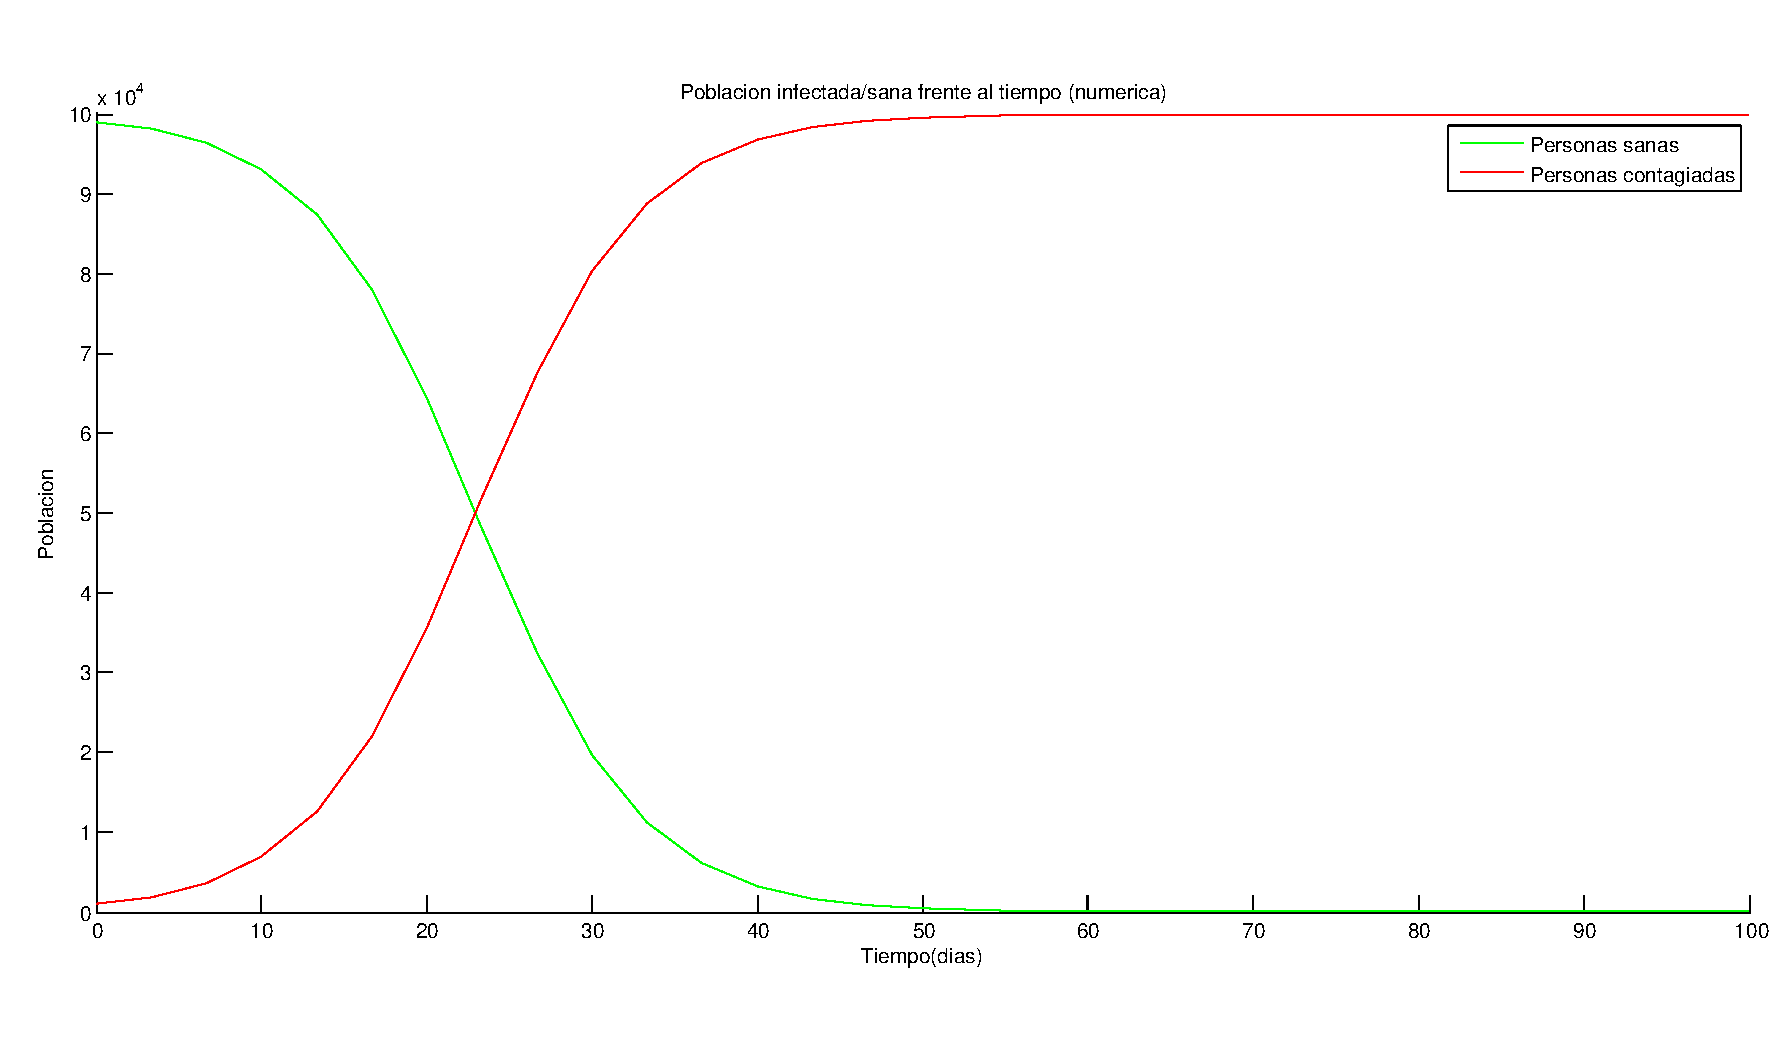
\includegraphics[width=1\textwidth]{grafica7.pdf}
	\caption{Población infectada/sana frente al tiempo (b=100)}
	\label{Fig:7}
\end{figure}

\indent Como puede observarse, los resultados teóricos que se obtuvieron en la Ecuación \ref{eq:limite} y los resultados gráficos cuando hacemos aumentar el límite máximo de días en nuestro modelo numérico son semejantes. En ambos casos cuando tendemos el tiempo al infinito se obtiene una cifra de contagios similar a la población total que estamos considerando.

\subsection{Enfermedad con eliminación de la población}
\indent Como vimos anteriormente, es imposible obtener solución analítica de nuestro problema, por lo que es un inconveniente a la hora de su cálculo numérico. El hecho de que tengamos su solución analítica nos permite comparar entre los resultados obtenidos por los dos métodos (analítico y numérico) y probar que ambos sean válidos si coinciden o se encuentran dentro de un intervalo de error que nosotros prefijamos. Por lo tanto antes este problema sólo nos queda sacar conclusiones de resultados obtenidos numéricamente. \\

\indent Con respecto a la gráfica que muestra la población eliminada con respecto del tiempo, Figura \ref{Fig:4}, cabe señalar que resulta un valor mucho más pequeño que la población total. Debido a esto su efecto en los primeros 30 días parece apenas apreciable, eliminando a tan sólo 80 personas de la población total. Aunque es un valor pequeño parece muy razonable, debido no sólo a los ya mencionados escasos días, sino también al pequeño valor que adquiere $ k_2 $ que representa la constante de eliminación de individuos como ya hemos mencionado anteriormente. \\

\indent Con respecto a la gráfica del estado de la población cabe decir que debido al escaso número de población que se encuentra eliminada parece no sufrir diferencias con respecto a nuestro primer problema \textit{Enfermedad sin eliminación de la población}. Por lo que la única solución factible que encuentro a la hora de comentar estos resultados es observar otra casuística. \\

\indent Así, primeramente vamos a aumentar el límite de tiempo máximo aplicado al problema, al igual que hemos hecho con el anterior problema \textit{Enfermedad sin eliminación de la población}. De ese modo vamos a representar por un lado la población que se elimina y por otro la población superviviente divida en personas sanas y personas infectadas. Así hacemos que la variable $ b $ adquiera el siguiente valor:
\begin{equation}
b=100000
\end{equation}

\indent Obteniendo las siguientes gráficas:
\begin{figure}[h!]
	\centering 		
	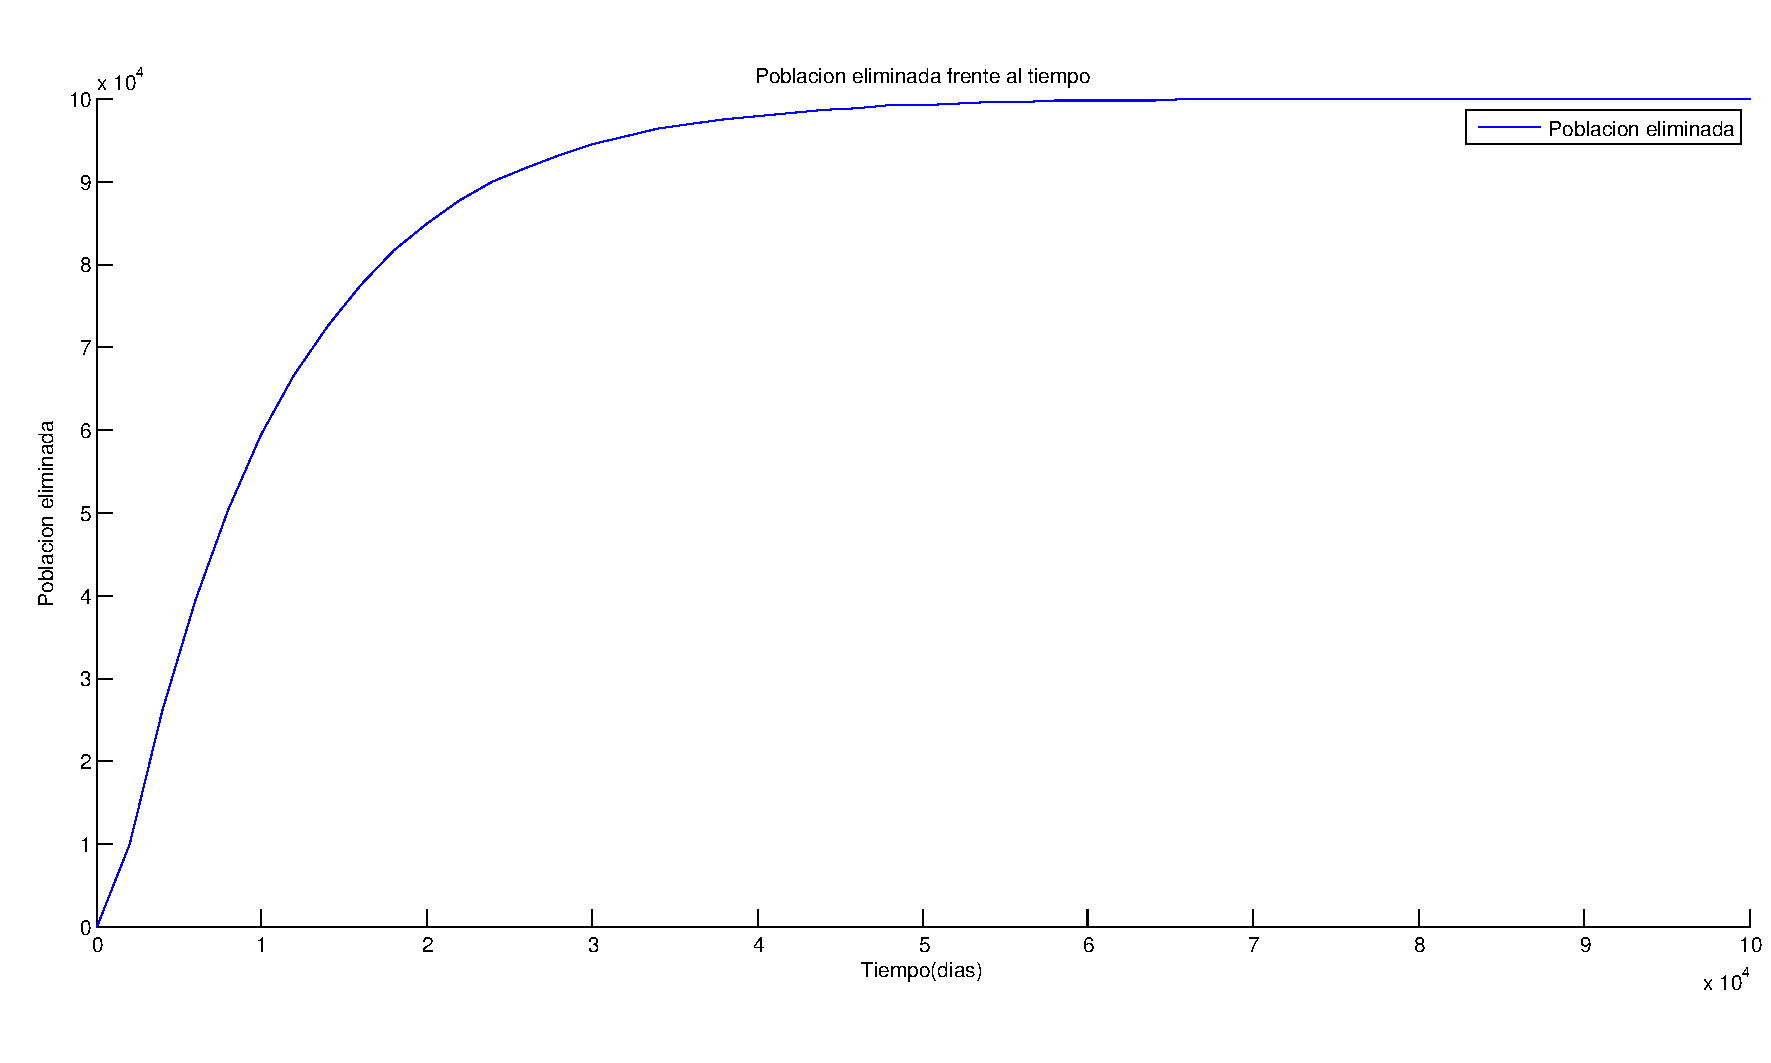
\includegraphics[width=1\textwidth]{grafica8.pdf}
	\caption{Población infectada/sana frente al tiempo (b=100000)}
	\label{Fig:8}
\end{figure}
\begin{figure}[h!]
	\centering 		
	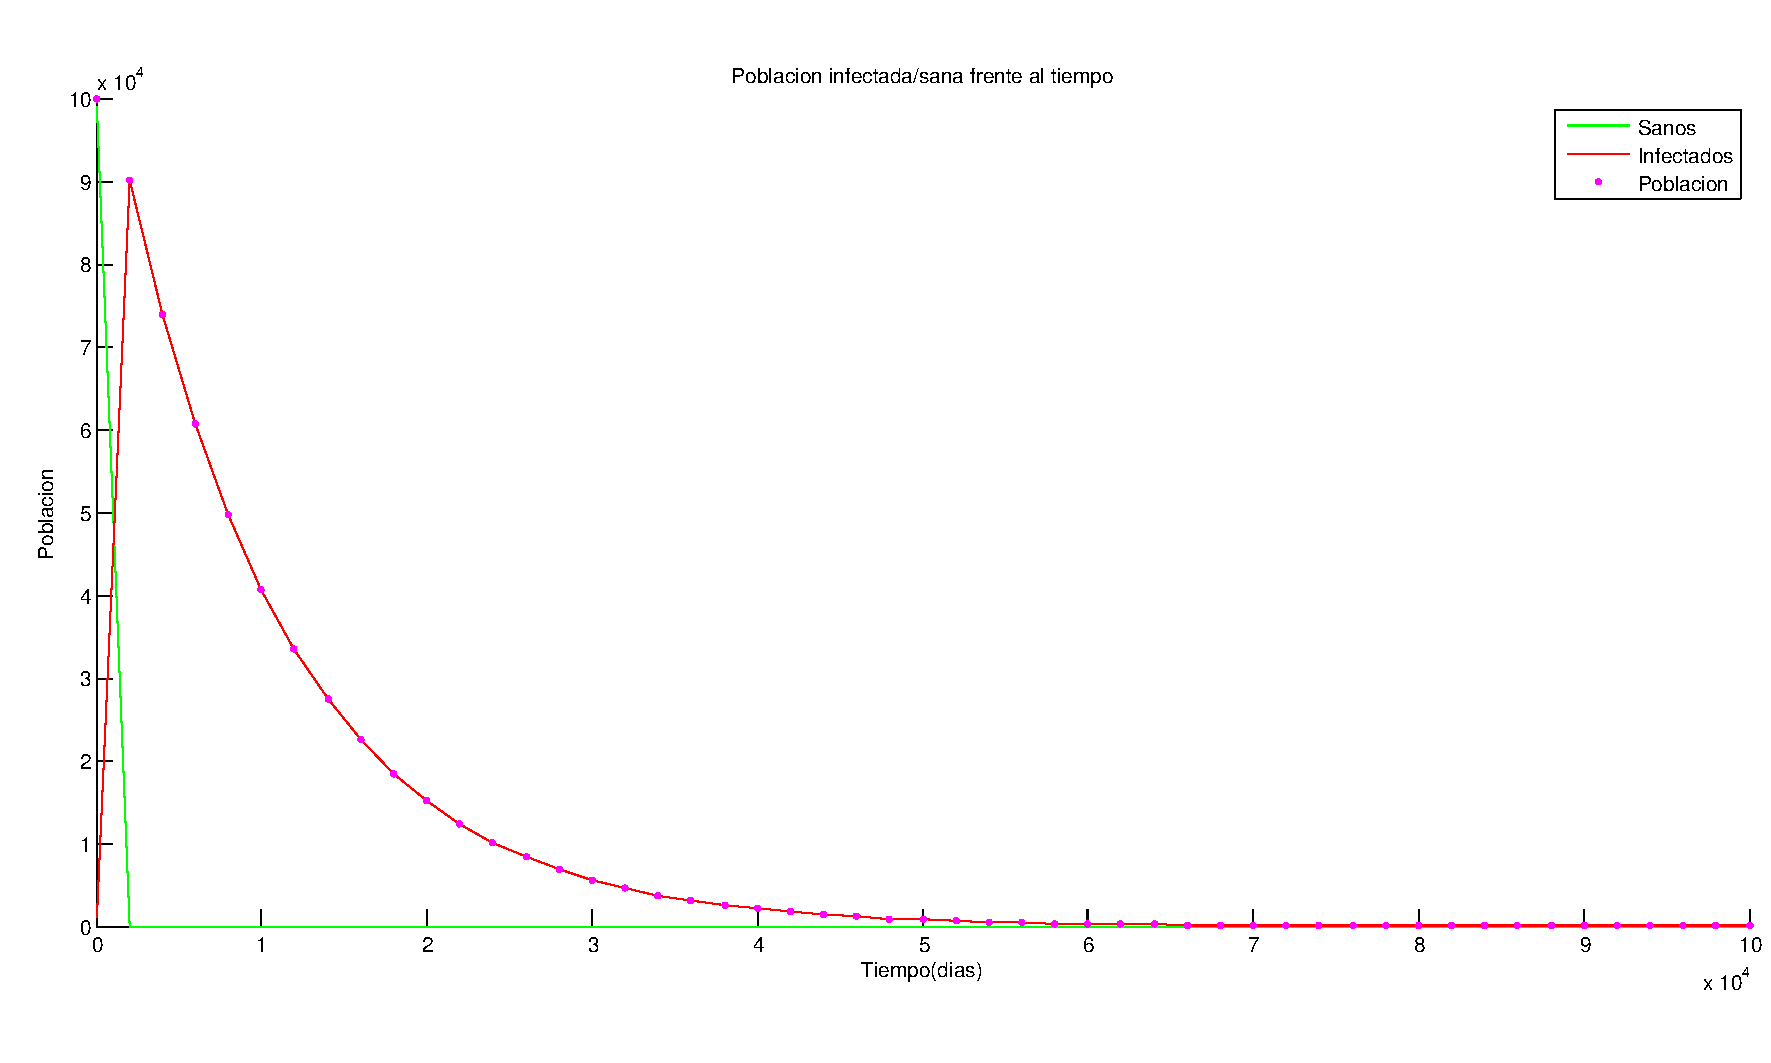
\includegraphics[width=1\textwidth]{grafica9.pdf}
	\caption{Población infectada/sana frente al tiempo (b=100000)}
	\label{Fig:9}
\end{figure}

\newpage
\indent Al igual que en el problema anterior, lo que acabamos de estudiar ha sido un límite para cuando el tiempo tiende a infinito. Puesto que no conocemos el valor analítico esta es nuestra única opción. Como puede observarse, la variable de población eliminada tiende a la población total cuando estudiamos el límite. Resultado esperado pues si se trata de una enfermedad que no tiene cura y es muy contagiosa la población al cabo de un cierto tiempo acabará muriendo. Razonamiento que se demuestra en la segunda gráfica. Se observa como rápidamente toda la población que ha sobrevivido hasta el momento ($ t\approx 300 $ días) se encuentra contagiada. A partir de entonces la número de personas y de gente infectada es similar. Es entonces cuando la población empieza a decaer. En un tiempo que tiende a infinito la población es nula. Resultado que esperábamos con el razonamiento de la primera gráfica. \\

\subsection{Comparación entre los dos problemas}
\indent Como ya hemos mencionado, la obtención del segundo problema de una población eliminada muy pequeña en los 30 primeros días hace que apenas se noten diferencias entre los valores de ambos problemas, Figura \ref{Fig:6}. En este caso, si en el último problema producimos una enfermedad mucho más virulenta y por lo tanto mortal modificando el valor de la \textit{constante de eliminación de la población} o $ k_2 $ obtendremos resultados mucho más significativos. Así podemos obtener la siguiente gráfica:
\begin{figure}[h!]
	\centering 		
	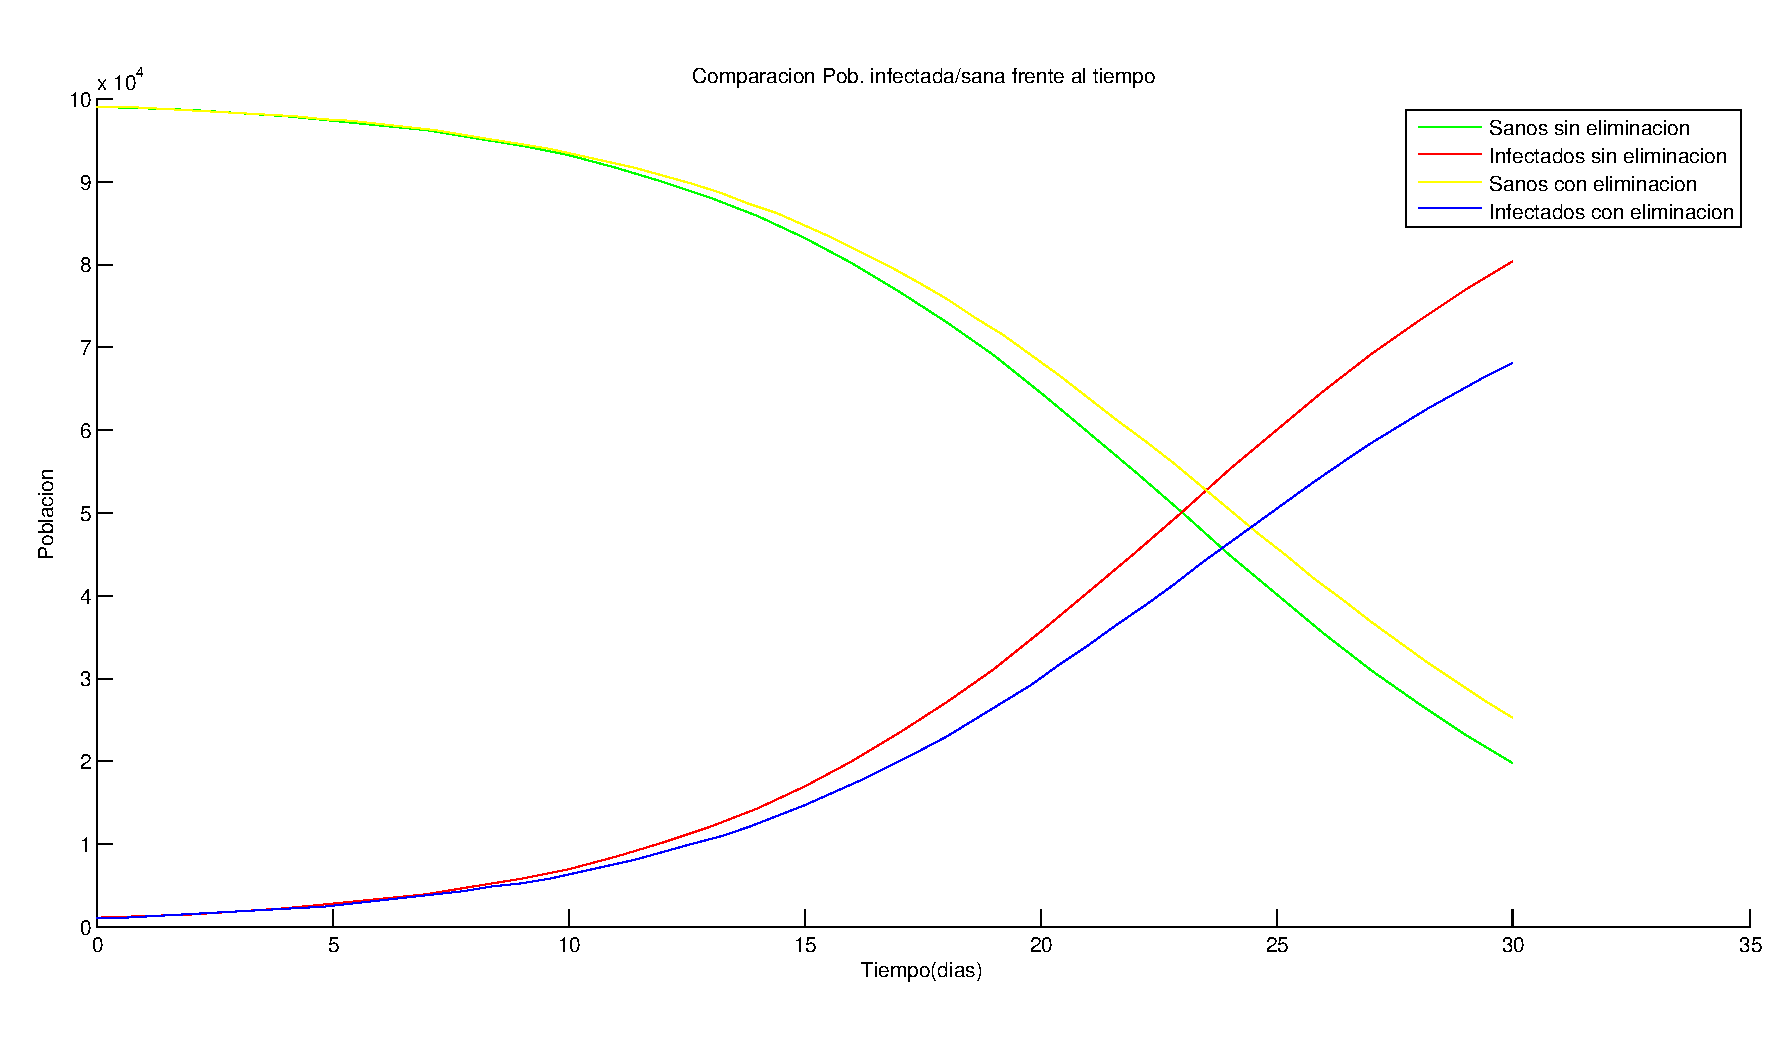
\includegraphics[width=1\textwidth]{grafica10.pdf}
	\caption{Comparación población infectada/sana frente al tiempo, siendo una más virulenta que otra.}
	\label{Fig:10}
\end{figure}

\indent En este caso la diferencia es mucho más notoria. Es por eso que existen problemas numéricos cotidianos que requieren un mayor nivel de abstracción. En nuestro caso los dos problemas planteados se podrían haber resuelto por cualquiera de los dos métodos expuestos. Pero si por el contrario hubiéramos tenido que controlar una población real de personas infectadas por una enfermedad muy grave el uso de un método u otro supone una diferencia de más de $ 10000 $ personas. Es por ello por lo que es muy importante el planteamiento de la resolución del problema y la elección de un método numérico adecuado. 


\newpage
\section{Caso Práctico: Pandemia de ébola en 2014}
\indent Durante el año de 2014 una pandemia del virus ébola azotó los hospitales de medio mundo sin poder encontrar freno alguno en su propagación. Se extendió desde África hacia casi todo el mundo. La utilización de métodos numéricos hubiera ayudado a su control y a su propagación.

\subsection{Antecedentes}
\indent La enfermedad del ébola es una enfermedad causada por el virus del ébola que se transmite por contacto con la sangre o los fluidos corporales con animales infectados(generalmente murciélagos) o personas contagiadas. Sus síntomas van desde simple dolores de cabeza o fiebre, hasta vómitos, fallos hepáticos y renales, hemorragias internas y por consiguiente la muerte. Es por ello por lo que se trata de una de las enfermedades más peligrosas en nuestro planeta.{\tiny \bf \textsuperscript{\cite{wikitres}}} \\

\indent En diciembre de 2013 se documentaba el primer caso de ébola en Guinea. Pero no fue hasta febrero de 2014 cuando la enfermedad se propagó por todo el país sin saberse aún las causas que lo producían dejando decenas de muertos. Las alarmas saltaron cuando en marzo de 2014 se informó de la primera muerte en Sierra Leona. No fue hasta finales de ese mismo mes cuando se produjeron las primeras muertes por contagio en Libia. A partir de entonces la enfermedad se contagió a otros países de África como Nigeria, Senegal o Malí. También se dieron casos puntuales en España, Italia, Francia, Reino Unido, Suiza, Estados Unidos, Noruega, Alemania y Holanda.{\tiny \bf \textsuperscript{\cite{wikicuatro}}}

\subsection{Descripción del problema}
\indent Debido al rápido contagio la utilización de métodos numéricos como los descritos anteriormente hubieran ayudado no sólo al control de la enfermedad sino a salvar vidas. Para ello me apoyo en datos consultados en la \textit{Organización Mundial de la Salud} (OMS){\tiny \bf \textsuperscript{\cite{wikicinco}}}{\tiny \bf \textsuperscript{\cite{oms}}}. Los cuales registraron los siguientes números de afectados y de víctimas:

\newpage	
\begin{table}[H]
	\centering
		\begin{tabular}{c|cc|cc|cc|cc}
\toprule
\bf FECHAS & \multicolumn{2}{c}{\bf TOTAL}  & \multicolumn{2}{c}{\bf Guinea} & \multicolumn{2}{c}{\bf Liberia} & \multicolumn{2}{c}{\bf Sierra Leona}  \\ 
			& Infec. & Vict. & Infec. & Vict. & Infec. & Vict. & Infec. & Vict. \\ \midrule
\bf 16 nov 2014		&\bf 15.145		&\bf 5.420	&	1.971&	1.192&	7.069& 	2.964&	6.073&	1.250				\\
\bf 11 nov 2014		&\bf 14.413		&\bf 5.177	&	1.919&	1.166&	6.878& 	2.812&	5.586&	1.187    			\\
\bf 9 nov 2014		&\bf 14.098		&\bf 5.160	&	1.878&	1.142&	6.822& 	2.836&	5.368&	1.169    			 \\
\bf 29 oct 2014		&\bf 12.567		&\bf 4.951	&	1.667&	1.018&	6.535& 	2.413&	5.338&	1.510     \\
\bf 23 oct 2014		&\bf 10.703		&\bf 4.922	&	1.553&	926	&	4.665& 	2.705&	3.896&	1.281      \\
\bf 20 oct 2014		&\bf 9.936		&\bf 4.877	&	1.540&	904	&	4.665& 	2.705&	3.706&	1.259       \\
\bf 14 oct 2014		&\bf 9.216		&\bf 4.555	&	1.519&	862	&	4.262& 	2.484&	3.410&	1.200       \\
\bf 12 oct 2014		&\bf 8.997		&\bf 4.493	&	1.472&	843	&	4.249& 	2.458&	3.252&	1.183       \\
\bf 8 oct 2014		&\bf 8.399		&\bf 4.033	&	1.350&	778	&	4.076& 	2.316&	2.950&	930          \\
\bf 5 oct 2014		&\bf 8.033		&\bf 3.865	&	1.298&	768	&	3.924& 	2.210&	2.789&	879          \\
\bf 1 oct 2014		&\bf 7.492		&\bf 3.439	&	1.199&	739	&	3.834& 	2.069&	2.437&	623          \\
\bf 28 sep 2014		&\bf 7.178		&\bf 3.338	&	1.157&	710	&	3.696&	1.998&	2.304&	622        \\
\bf 23 sep 2014		&\bf 6.574		&\bf 3.091	&	1.074&	648	&	3.458& 	1.830&	2.021&	605       \\
\bf 21 sep 2014		&\bf 6.263		&\bf 2.917	&	1.022&	635	&	3.280& 	1.677&	1.940&	597       \\
\bf 19 sep 2014		&\bf 5.864		&\bf 2.811	&	1.008&	632	&	3.022& 	1.578&	1.813&	593       \\
\bf 14 sep 2014		&\bf 5.347		&\bf 2.630	&	942	&	601	&	2.710&	1.459&	1.673&	562         \\
\bf 6 sep 2014		&\bf 4.293		&\bf 2.296	&	862	&	555	&	2.046&	1.224&	1.361&	509          \\
\bf 31 ago 2014		&\bf 3.707		&\bf 1.848	&	771	&	494	&	1.698&	871	&	1.216&	476             \\
\bf 25 ago 2014		&\bf 3.071		&\bf 1.553	&	648	&	430	&	1.378&	694	&	1.026&	422             \\
\bf 20 ago 2014		&\bf 2.615		&\bf 1.427	&	607	&	406	&	1.082&	624	&	910	&	392\\
\bf 18 ago 2014		&\bf 2.473		&\bf 1.350	&	579	&	396	&	972	&	576	&	907	&	374 \\
\bf 16 ago 2014		&\bf 2.240		&\bf 1.229	&	543	&	394	&	834	&	466	&	848	&	365 \\
\bf 13 ago 2014		&\bf 2.127		&\bf 1.145	&	519	&	380	&	786	&	413	&	810	&	348 \\
\bf 11 ago 2014		&\bf 1.975		&\bf 1.069	&	510	&	377	&	670	&	355	&	783	&	334 \\
\bf 9 ago 2014		&\bf 1.848		&\bf 1.013	&	506	&	373	&	599	&	323	&	730	&	315  \\
\bf 6 ago 2014		&\bf 1.779		&\bf 961	&	495	&	367	&	554	&	294	&	717	&	298   \\
\bf 4 ago 2014		&\bf 1.711		&\bf 932	&	495	&	363	&	516	&	282	&	691	&	286   \\
\bf 1 ago 2014		&\bf 1.603		&\bf 887	&	485	&	358	&	468	&	255	&	646	&	273   \\
\bf 30 jul 2014		&\bf 1.440		&\bf 826	&	472	&	346	&	391	&	227	&	574	&	252   \\
\bf 27 jul 2014		&\bf 1.323		&\bf 729	&	460	&	339	&	329	&	156	&	533	&	233   \\
\bf 23 jul 2014		&\bf 1.201		&\bf 672	&	427	&	319	&	249	&	129	&	525	&	224   \\
\bf 20 jul 2014		&\bf 1.093		&\bf 660	&	415	&	314	&	224	&	127	&	454	&	219   \\
\bf 17 jul 2014		&\bf 1.048		&\bf 632	&	410	&	310	&	196	&	116	&	442	&	206   \\
\bf 14 jul 2014		&\bf 982		&\bf 613	&	411	&	310	&	174	&	106	&	397	&	197     \\
\bf 12 jul 2014		&\bf 964		&\bf 603	&	406	&	304	&	172	&	105	&	386	&	194\\
\bf 8 jul 2014		&\bf 888		&\bf 539	&	409	&	309	&	142	&	88	&	337	&	142  \\
\bf 6 jul 2014		&\bf 944		&\bf 518	&	408	&	307	&	131	&	84	&	305	&	127  \\
\bf 2 jul 2014		&\bf 779		&\bf 481	&	412	&	305	&	115	&	75	&	252	&	101  \\
\bf 30 jun 2014		&\bf 759		&\bf 467	&	413	&	303	&	107	&	65	&	239	&	99  \\
\bf 20 jun 2014		&\bf 599		&\bf 353	&	390	&	270	&	51	&	34	&	158	&	49   \\
\bf 17 jun 2014		&\bf 528		&\bf 337	&	398	&	264	&	33	&	24	&	97	&	49    \\
\bf 5 jun 2014		&\bf 452		&\bf 242	&	351	&	226	&	12	&	9	&	89	&	7       \\
\end{tabular}
\end{table}
\newpage
\begin{table}[H]
\centering
\begin{tabular}{c|cc|cc|cc|cc}
\toprule
\bf FECHAS & \multicolumn{2}{c}{\bf TOTAL}  & \multicolumn{2}{c}{\bf Guinea} & \multicolumn{2}{c}{\bf Liberia} & \multicolumn{2}{c}{\bf Sierra Leona}  \\ 
& Infec. & Vict. & Infec. & Vict. & Infec. & Vict. & Infec. & Vict. \\ \midrule
\bf 29 may 2014			&\bf 337		&\bf 207	&	291	&	193	&	12	&	9	&	34	&	5       \\
\bf 27 may 2014			&\bf 309		&\bf 200	&	281	&	186	&	12	&	9	&	16	&	5       \\
\bf 23 may 2014			&\bf 270		&\bf 183	&	258	&	174	&	12	&	9	&	0	&	0        \\
\bf 18 may 2014			&\bf 265		&\bf 185	&	253	&	176	&	12	&	9	&	0	&	0        \\
\bf 12 may 2014			&\bf 260		&\bf 182	&	248	&	171	&	12	&	11	&	0	&	0       \\
\bf 10 may 2014			&\bf 245		&\bf 168	&	233	&	157	&	12	&	11	&	0	&	0       \\
\bf 3 may 2014			&\bf 266		&\bf 166	&	231	&	155	&	35	&	11	&	0	&	0		\\
\bf 24 abr 2014			&\bf 253		&\bf 152	&	218	&	141	&	35	&	11	&	0	&	0	\\
\bf 21 abr 2014			&\bf 242		&\bf 147	&	208	&	136	&	34	&	11	&	0	&	0	\\
\bf 17 abr 2014			&\bf 230		&\bf 142	&	203	&	129	&	27	&	13	&	0	&	0	\\
\bf 16 abr 2014			&\bf 224		&\bf 135	&	197	&	122	&	27	&	13	&	0	&	0 \\
\bf 14 abr 2014			&\bf 194		&\bf 121	&	168	&	108	&	26	&	13	&	0	&	0 \\
\bf 10 abr 2014			&\bf 183		&\bf 113	&	158	&	101	&	25	&	12	&	0	&	0 \\
\bf 7 abr 2014			&\bf 167		&\bf 105	&	151	&	95	&	16	&	10	&	0	&	0   \\
\bf 1 abr 2014			&\bf 135		&\bf 88		&	127	&	83	&	8	&	5	&	0	&	0      \\
\bf 31 mar 2014			&\bf 130		&\bf 82		&	122	&	80	&	8	&	2	&	0	&	0     \\
\bf 27 mar 2014			&\bf 103		&\bf 66		&	103	&	66	&	0	&	0	&	0	&	0     \\
\bf 26 mar 2014			&\bf 86			&\bf 62		&	86	&	62	&	0	&	0	&	0	&	0      \\
\bf 24 mar 2014			&\bf 86			&\bf 59		&	86	&	59	&	0	&	0	&	0	&	0      \\
\bf 22 mar 2014			&\bf 49			&\bf 29		&	49	&	29	&	0	&	0	&	0	&	0	     \\
\end{tabular}
\caption{Datos de población infectada y fallecida a causa del Ébola en el África Occidental}
\end{table}

\indent Nuestro estudio se va a basar en la población infectada, no en la fallecida. Ya que entre los tres países suman una población de 19 millones de personas{\tiny \bf \textsuperscript{\cite{guinea}}}{\tiny \bf \textsuperscript{\cite{sierraleona}}}{\tiny \bf \textsuperscript{\cite{liberia}}}, siendo el número de fallecidos notoriamente menor. Si lo considerásemos tendríamos el caso de \textit{Enfermedad con eliminación de la población} pero tendríamos el mismo problema que nos ha surgido donde el número de población eliminada era muy inferior, por lo que la población apenas descendía. Debido a eso vamos a realizar una aproximación del primer tipo \textit{Enfermedad sin eliminación de la población}.\\

\indent Para ello debemos determinar algunas variables de antemano. Para la variable del tiempo, que en nuestro caso llamaremos \texttt{dias} la he tomado contando los días desde el primero que es el 0, mientras que las personas contagiadas se denominan \texttt{infec} cuyos valores están sacados directamente de la tabla. Para la tasa de contagio $ k $ basta hacer una regresión exponencial con alguna herramienta de cálculo como Microsoft Excel y haciendo una operación sencilla se obtiene un valor aproximado de:
\begin{equation}
k=1.37\cdot 10^(-9)
\end{equation}

\indent El resto de variables están sacadas directamente de la tabla o de valores conocidos que ya hemos mencionado: 
\begin{equation}
y_0=49
\end{equation}
\begin{equation}
pob=19\cdot 10^{6}
\end{equation}

\subsection{Código}
\indent Código correspondiente al archivo \texttt{ebola.m}
\lstinputlisting{ebola.m}

\subsection{Resultados numéricos}
\indent De ese modo obtenemos la siguiente representación:
\begin{figure}[h!]
	\centering 		
	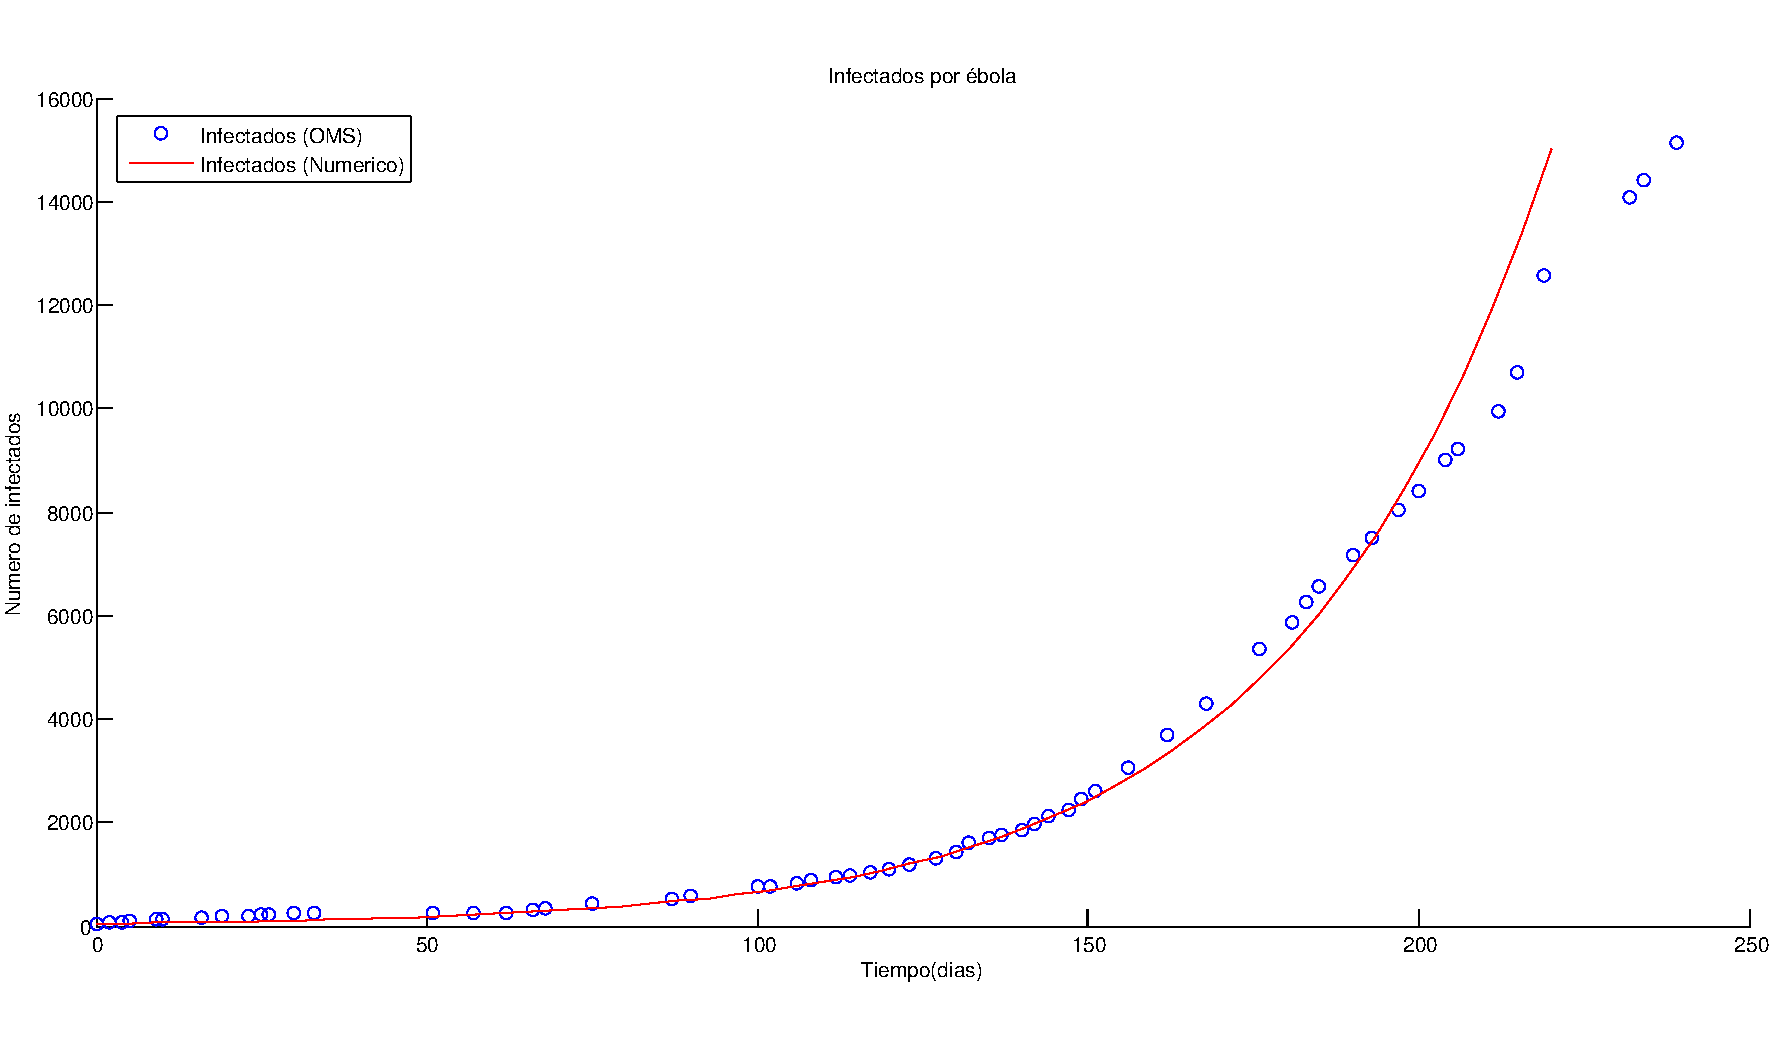
\includegraphics[width=1\textwidth]{grafica11.pdf}
	\caption{Estudio de los infectados por ébola en el África Occidental}
	\label{Fig:11}
\end{figure}

\indent Como vemos excepto en los puntos extremales, el método numérico aproxima muy bien los valores dados por la OMS y por tanto reales. Como dijimos en su momento en la sección \textit{Comentarios acerca de los programas}, este programa en concreto presenta muchísima inestabilidad numérica debido a la alta población que se le ha introducido. Un cambio en un sólo decimal de la \textit{tasa de contagio} hace que el programa origine valores que para nada se aproximan a lo conocido. A pesar de ello, el resultado es más que satisfactorio, ya que no sólo aproxima bastante bien los puntos sino que también se trata de un problema real y el hecho de encontrar un método numérico que se aproxime lo suficiente puede ser incluso la peor parte del problema.

\newpage
	\addcontentsline{lot}{section}{Referencias}
	\bibliographystyle{unsrt}
	\bibliography{biblo}	
\end{document}
